\documentclass[a4paper, 11pt]{article}

% Nécessaire
\usepackage[french]{babel}
\usepackage[utf8]{inputenc}
\usepackage[T1]{fontenc}
\usepackage{lmodern}
\usepackage{amsmath, amsthm}
\usepackage{amsfonts,amssymb}

% Marge
\usepackage{geometry}
\geometry{margin={2.2cm ,2cm}}

% Figures, graphiques
\usepackage{graphicx}
\usepackage{epsfig}
\usepackage{caption}

% Surlignage
\usepackage{alltt}

\usepackage{xcolor}
\usepackage{soul}
\usepackage{color}
\usepackage{colortbl}

% Indicatrice
\usepackage{dsfont}

\usepackage{multirow}
\usepackage{eurosym}
\usepackage{extarrows}

% Graphique
\usepackage{tikz}


% Titre
\title{Récapitulatif de ce qui a été fait avec Mohammed}
\author{}
\date{}



\begin{document}
\maketitle

Les résultats obtenus jusqu'à présent possédaient trois problèmes majeurs :
\begin{itemize}
 \item la proportion d'individus exogènes était largement supérieure à la proportion d'individus émergents ;
 \item une difficulté en prendre en compte la chute finale ;
 \item un paramètre $\mu_{EH}$ presque exclusivement calibré à 0 par l'algorithme NSGA-II.
\end{itemize}
L'analyse de sensibilité réalisée au préalable a montré l'absence d'impact du paramètre $\mu_{EH}$ sur deux des trois critères. D'une importance négligeable vis à vis du modèle dans son ensemble, la calibration de ce paramètre et son importance n'étaient pas bien prise en compte par NSGA-II. Ce dernier préférant ajuster les estimations avec $\gamma$, seul paramètre permettant une chute en fin de saison --- et par là même donnant une très grande place aux exogènes au détriment des émergents.

Une idée fût donc d'introduire un nouveau critère pour modéliser la préférence des individus émergents par rapport aux exogènes, permettant \textit{a priori} de régler deux des trois problèmes précédemment mentionnés.


\section{Mise en œuvre}

Pour ce faire, il n'est pas possible de rajouter le nouveau critère en plus des trois autres; NSGA-II ne fonctionnant pas au-delà de trois critères. Il a donc fallu enlever un critère pour le remplacer par le nouveau. La fonction de coût utilisée est la $NRMSE$ définie par
$$
NRMSE(y, \hat y) = \frac{\sqrt{\frac{1}{N} \sum_{j=1}^N \left( y_j -\hat y_j \right)^2 }}{\max(y) - \min(y)}.
$$
Avec cette fonction de coût (et non plus la fonction $MAE$), on a lancé 5 répétitions de NSGA-II (\emph{popsize} = 100 et \emph{generations} = 200). On a ainsi pu récupérer 500 solutions accompagnés de la valeur de la $NRMSE$ produite sur chaque sous-bloc. Les corrélations trouvés sur ces valeurs sont les suivantes :
$$
\rho\left( ER, PS \right) = -0.869 \qquad \rho\left( ER, EH \right) = 0.761 \qquad \rho\left(PS, EH \right) = -0.943
$$
Les sous-blocs PS et EH sont très corrélés négativement. Baisser l'erreur de l'un entraîne une augmentation de l'autre. Comme le montre la figure~\ref{fig:cost} l'erreur associée à EH est plus grande que celle associée à PS. En retirant le critère PS, cela contribuera à baisser l'erreur sur l'enherbement haut de sorte que les erreurs entre PS et EH seront plus équilibrées. Cela libère également un critère permettant d'introduire notre nouveau critère.

\begin{figure}[ht]
 \centering
 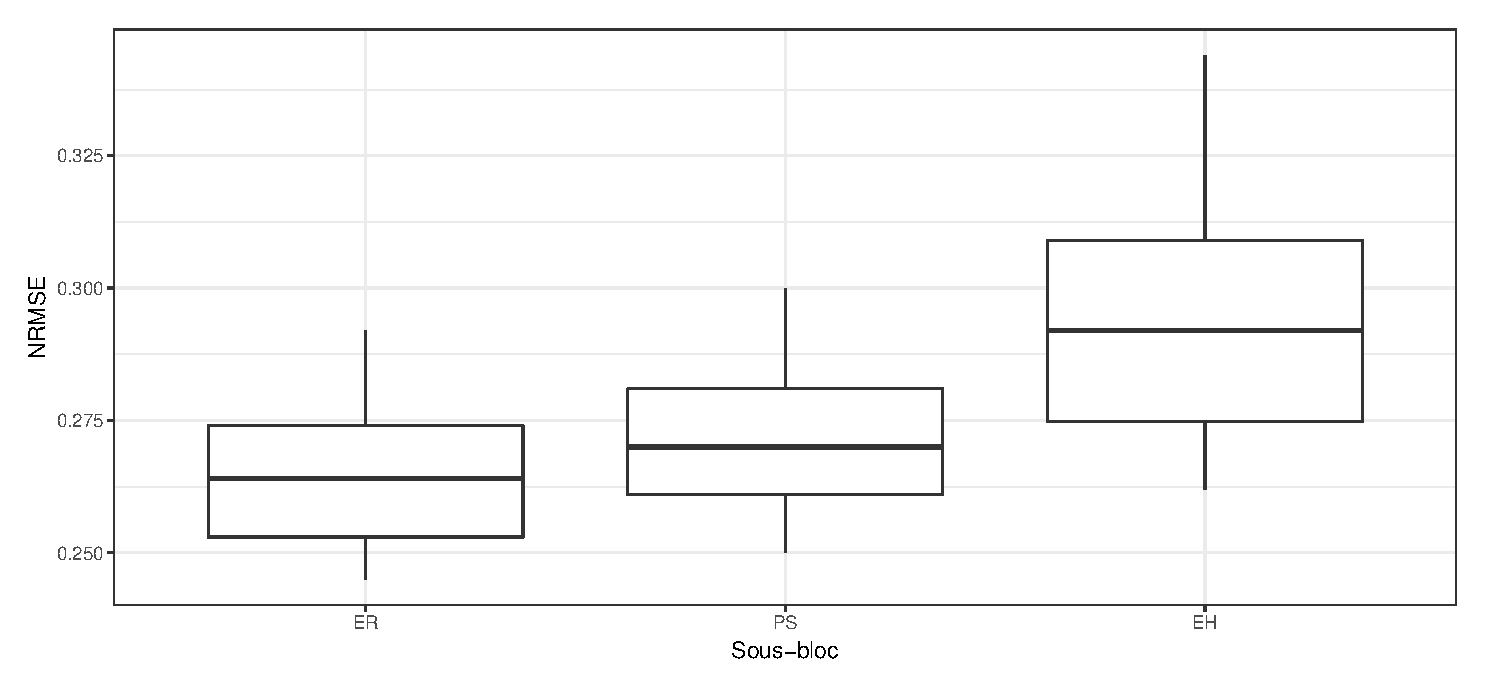
\epsfig{file = plots/comp_cost.eps, scale = 0.65}
 \caption{Comparaison des valeurs de la NRMSE des solutions proposées par NSGA-II en fonction des trois sous-blocs.}
 \label{fig:cost}
\end{figure}



Ce nouveau critère portant sur la préférence des émergents est défini par 
$$
\max \sum_{t, i}\frac{N_{t,i} - N_{t, i}^{\text{exo}}}{N_{t, i}}.
$$
Nos trois critères sont donc maintenant : ER, EH et la maximisation des émergents.


\section{Calibration}

Pour la calibration des paramètres en fonction de nos trois critères, on relance NSGA-II 5 fois avec une taille de population de 100. Il s'avère que parmi les 500 solutions certaines sont dominées par d'autres. Au final, il nous reste 317 solutions.

Choisir la solution qui minimise la distance à 0 n'est pas toujours la solution la plus pertinente vis à vis de notre problème. Il peut être intéressant de rechercher, d'explorer parmi les solutions proposées. À cette fin, effectuer une ACP peut s'avérer intéressant (voire une ACP-VI). Ce fût chose faite. Les deux premiers axes capturent près de 91\% de l'inertie. Les représentations des individus et des variables sont visibles sur la figure~\ref{fig:pca}. On remarque d'emblée que certaines de nos solutions (les individus dans l'ACP) privélgient un critère aux autres. \textit{A priori} ces solutions-là ne sont pas celles qui nous intéresse le plus, vu que l'on voudrait plutôt des paramètres qui ne négligent aucun des critères; nous sommes donc plus à la recherche d'un compromis. Certaines des paramètres sont corrélés à nos critères. Ainsi le paramètre $\mu_{EH}$ est corrélé au critère ER et le critère de préférence des endogènes est corrélé à $\gamma$. Le critère ER est quant à lui plus ou moins corrélé au paramètre $\mu_{ER}$.


\begin{figure}[ht]
 \centering
 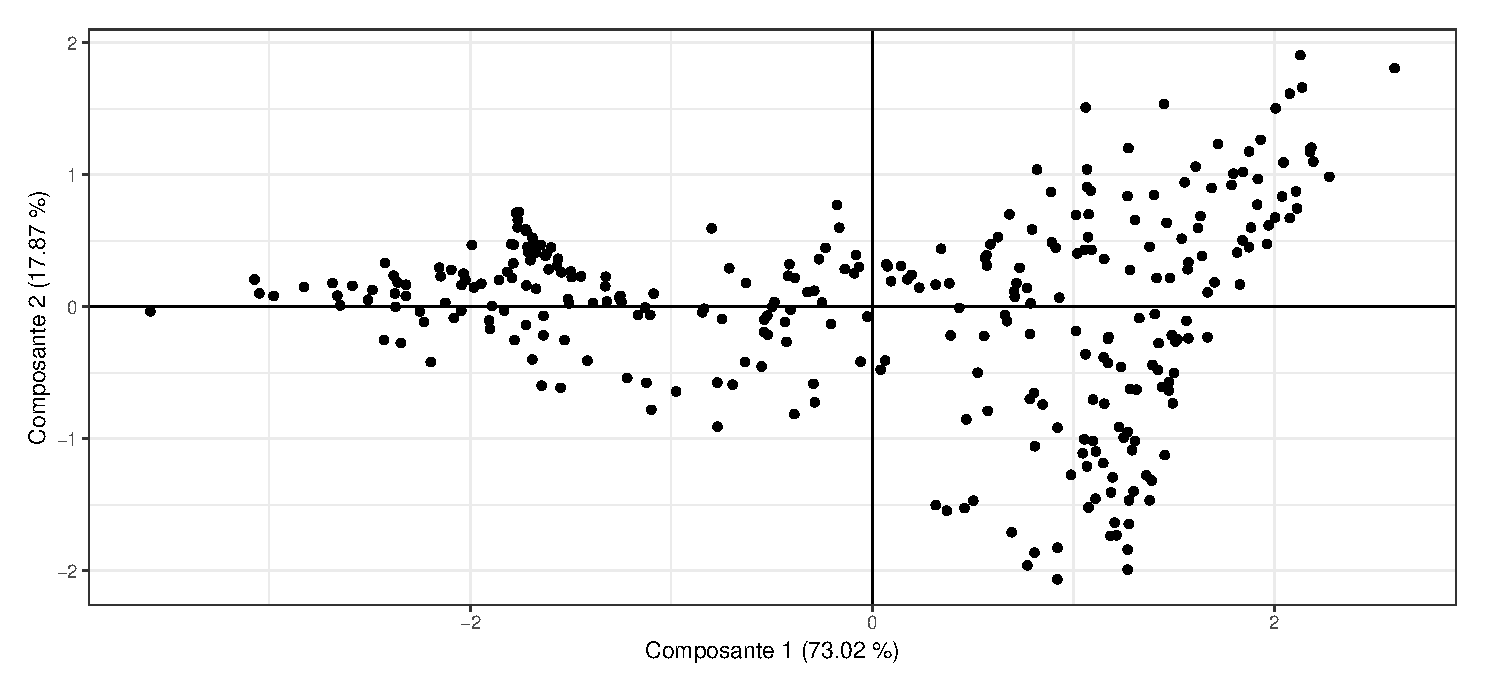
\epsfig{file = plots/pca_nsga_ind.eps, scale = 0.65}
 
 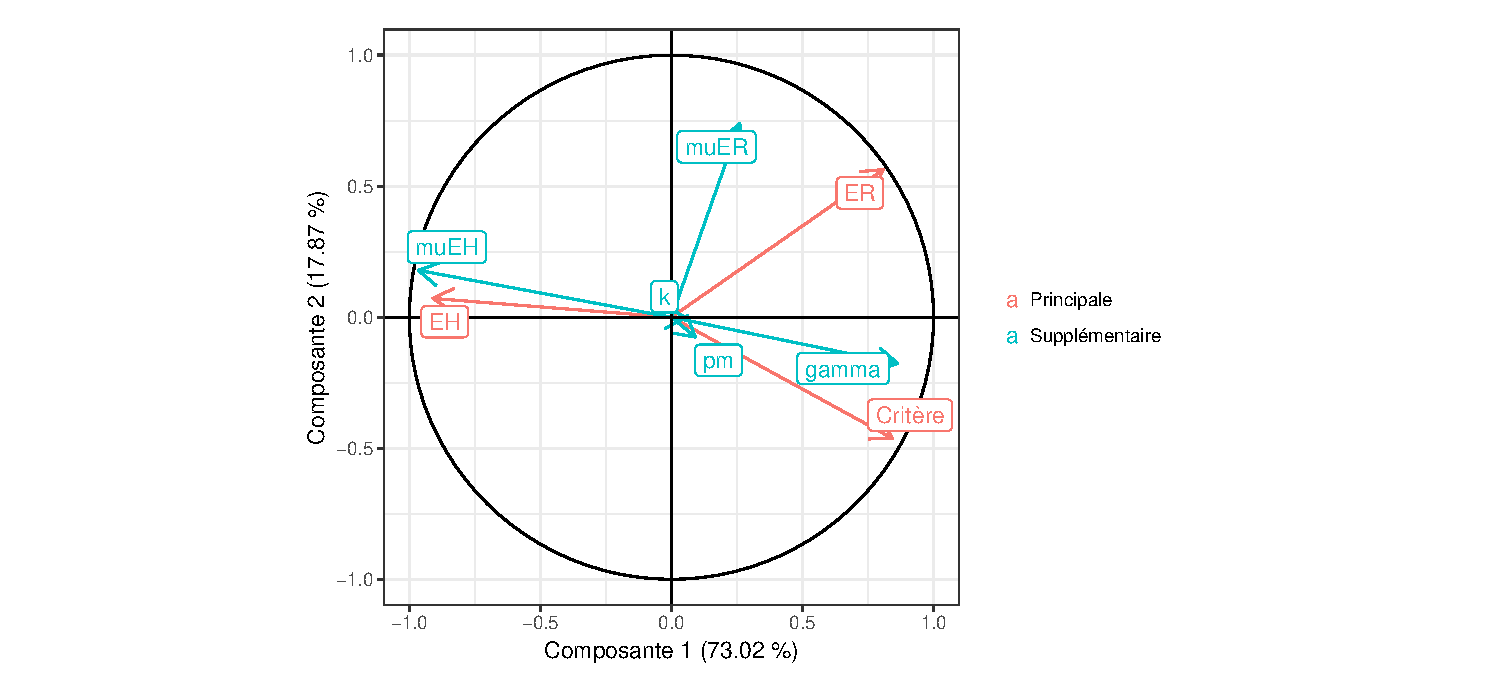
\epsfig{file = plots/pca_nsga_var.eps, scale = 0.65}
 
 \caption{Repésentation des individus (en haut) et des variables (en bas) sur le plan (1,2).}
 
 \label{fig:pca}
\end{figure}


D'après l'ACP, un bon jeu de paramètre maximiserait $\mu_{ER}$ et $\mu_{EH}$ et qui minimiserait $\gamma$; ces trois paramètres étant les plus corrélés à nos trois critères.
En regardant les paramètres qui ont :
\begin{itemize}
 \item un $\mu_{ER}$ supérieur à la médiane des $\mu_{ER}$ de toutes les solutions ;
 \item un $\mu_{EH}$ supérieur à la médiane des $\mu_{EH}$ de toutes les solutions ;
 \item un $\gamma$ inférieur à la médiane des $\gamma$ de toutes les solutions ;
 \item un $p_m$ supérieur à la médiane des $p_m$ de toutes les solutions;
\end{itemize}
seules 35 solutions demeuraient.

Parmi ces solutions, on essaye deux jeux de paramètres : celui qui minimise la norme 1 et celui correspondant à la moyenne des 35 solutions. Les paramètres sont
{%
\newcommand{\mc}[3]{\multicolumn{#1}{#2}{#3}}
\begin{center}
\begin{tabular}{lllll}
\mc{5}{c}{Min $\|\cdot \|_1$}\\
$\gamma$ & $p_m$ & $\mu_{ER}$ & $\mu_{EH}$ & $k$\\
0.042 & 0.960 & 0.999 & 0.408 & 1.563\\
\mc{5}{c}{Moyenne}\\
$\gamma$ & $p_m$ & $\mu_{ER}$ & $\mu_{EH}$ & $k$\\
0.031 & 0.978 & 0.981 & 0.625 & 20.760
\end{tabular}
\end{center}
}%
Les dynamiques associées sont visibles sur la figure~\ref{fig:dyn}.
\begin{figure}[ht]
 \centering
 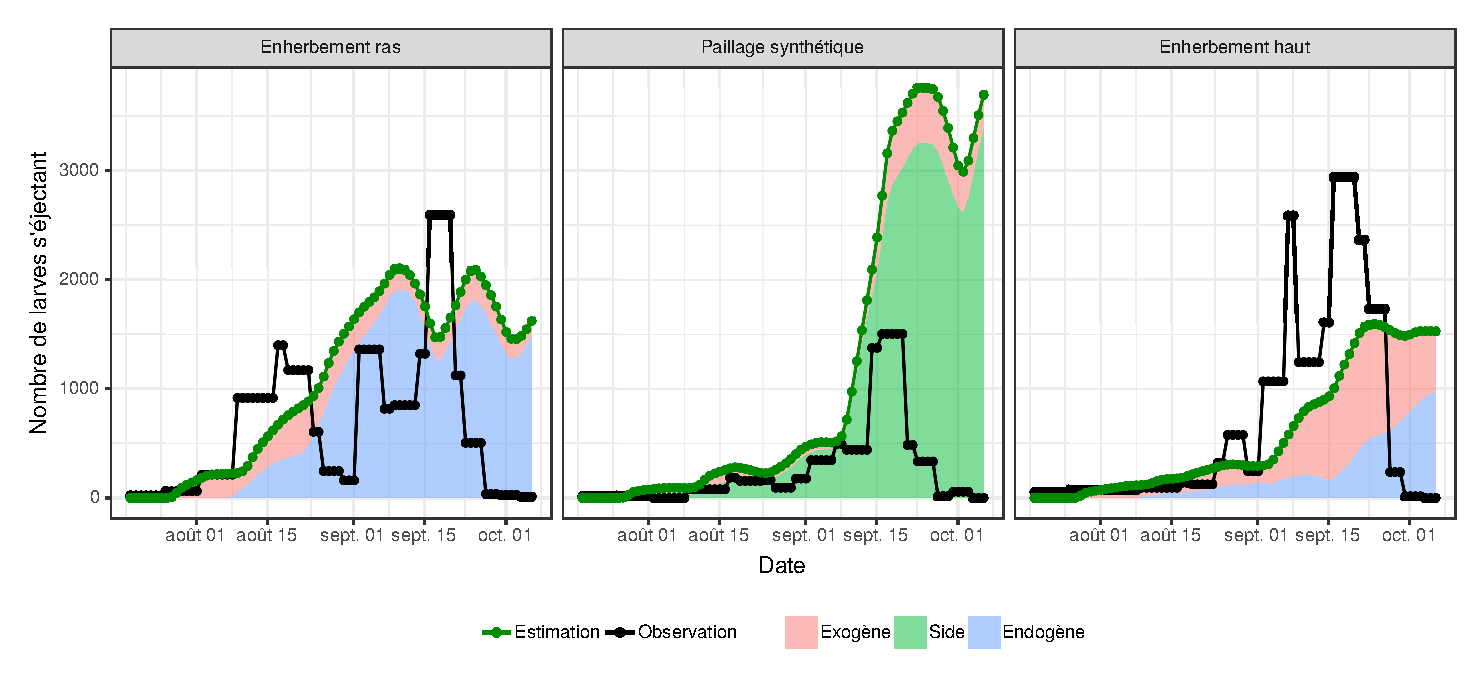
\epsfig{file = plots/arg1.eps, scale = 0.65}
 
 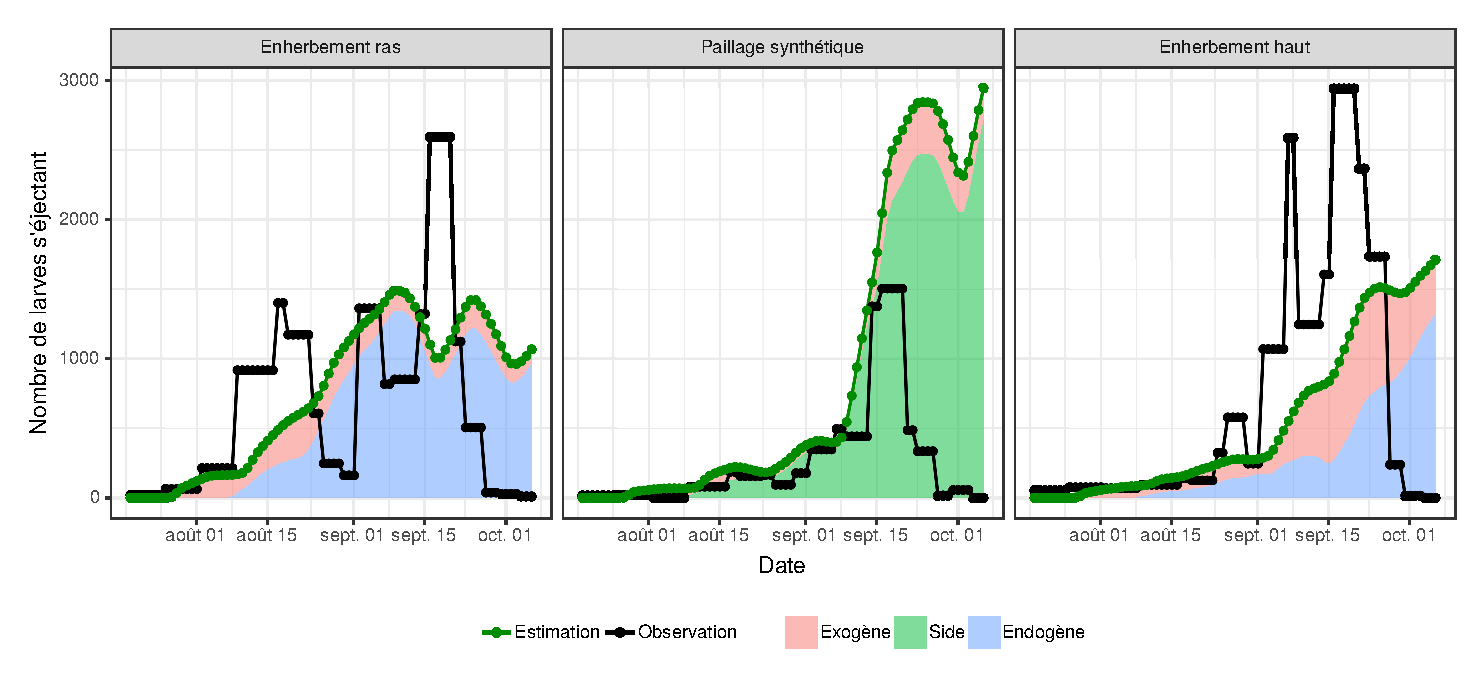
\epsfig{file = plots/arg2.eps, scale = 0.65}
 
 \caption{Dynamiques produites par la minimisation de la norme 1 (en haut) et par la moyenne des solutions retenues (en bas).}
 
 \label{fig:dyn}
\end{figure}

On remarque que la proportion d'endogène est supérieure à celle d'exogène. On remarque la présence d'endogène dans la parcelle avec un enherbement haut. Un autre problème est cependant apparu sur la parcelle bachée : les valeurs estimées sont bien supérieures aux valeurs observées. Pour pallier ce problème, on peut rajouter la contrainte
$$
\max_t L_{t, PS} \leq 1500
$$
au problème.

Une autre aprroche consiste à continuer à explorer les solutions pour en trouver une qui conviendrait mieux. Un exemple est visible sur la figure~\ref{arg5}.

\begin{figure}[ht]
 \centering
 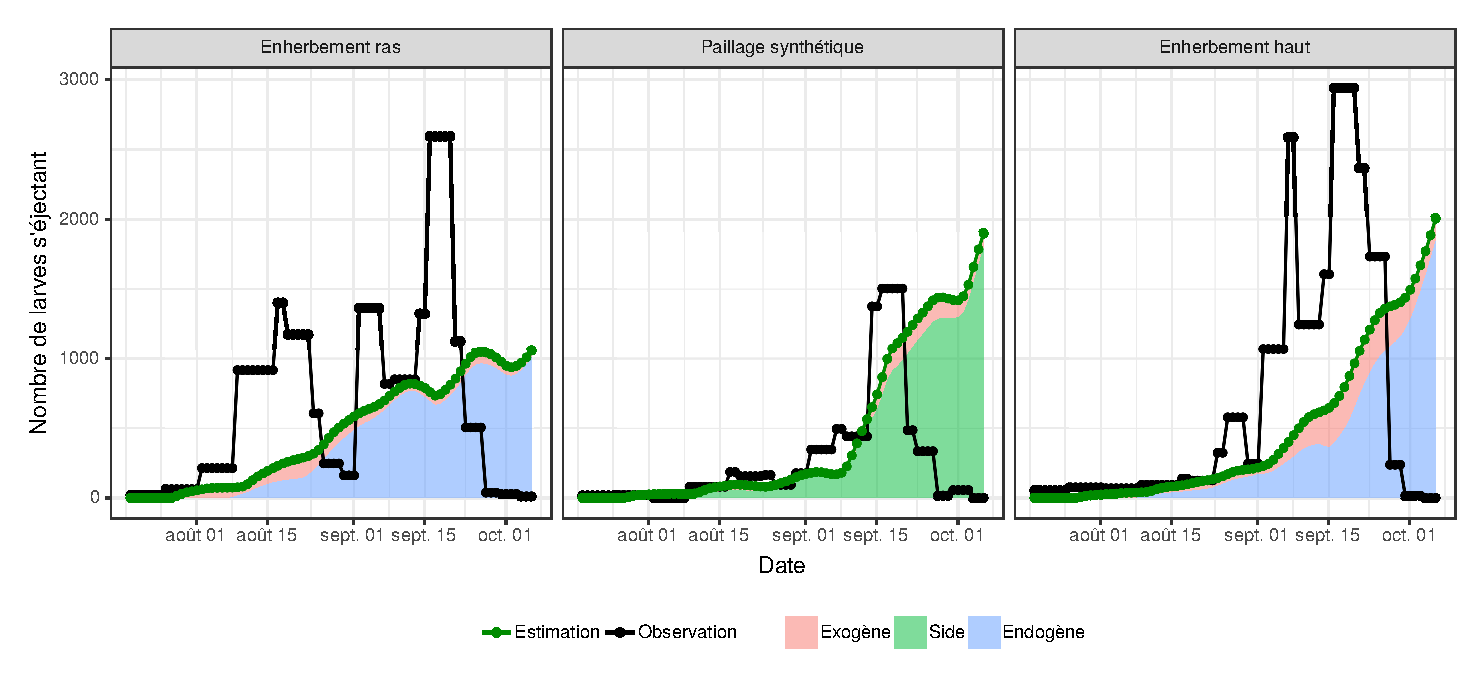
\epsfig{file = plots/arg5.eps, scale = 0.65}
 \caption{Dynamiques produites en utilisant les arguments $\gamma = 0.014$, $p_m = 0.746$, $\mu_{ER} = 1.000$, $\mu_{EH} = 1.000$ et $k = 2.264$}
 \label{arg5}
\end{figure}


\section{Autres résultats notables}

L'analyse de sensibilité doit se faire avant la calibration. 

Le $\mu_{global}$ ayant un impact relativement fort sur le modèle, il serait bon d'inclure ce paramètre dans la calibration (en restant autour de la valeur de la littérature).

La fonction de coût $MAE$ a été remplacée par la fonction de coût $NRMSE$. Cette dernière a l'avantage d'être normalisée ce qui rend les comparaisons possibles.



\newpage
\clearpage

Proportion partant de $i$ vers $j$

$$
p_m \frac{I_j}{I_i + I_j + dI_k}
$$


Proportion partant de $i$ vers $k$

$$
p_m \frac{dI_k}{I_i + I_j + dI_k}
$$

Proportion restant dans $i$

$$
(1 - p_m) + p_m \frac{I_i}{I_i + I_j + dI_k}
$$



\end{document}

